%%%%%%%%%%%%%%%%%%%%%%%%%%%%%%%%%%%%%%%%c
% Beamer Presentation
% LaTeX Template
% Version 1.0 (10/11/12)
%
% This template has been downloaded from:
% http://www.LaTeXTemplates.com
%
% License:
% CC BY-NC-SA 3.0 (http://creativecommons.org/licenses/by-nc-sa/3.0/)
%
%%%%%%%%%%%%%%%%%%%%%%%%%%%%%%%%%%%%%%%%%

%----------------------------------------------------------------------------------------
%	PACKAGES AND THEMES
%----------------------------------------------------------------------------------------

\documentclass[landscape, aspectratio=169]{beamer}

\newcommand{\fullimage}[2][]{
{ % all template changes are local to this group.
        \begin{tikzpicture}[remember picture,overlay]
            \node[at=(current page.center)] {
                \includegraphics[width=\paperwidth, height=.95\paperheight, keepaspectratio]{#2}}; 
            \node[at=(current page.south), yshift=0.2cm]{\colorbox{uclbleunuit}{\scriptsize#1}};
          \end{tikzpicture}
}
}

\newcommand{\fullimageb}[2][]{
{ % all template changes are local to this group.
        \begin{tikzpicture}[remember picture,overlay]
            \node[at=(current page.center)] {
                \colorbox{white}{\includegraphics[width=\paperwidth, height=.95\paperheight, keepaspectratio]{#2}}};
            \node[at=(current page.south), yshift=0.2cm] {\colorbox{uclbleunuit}{\scriptsize#1}};
          \end{tikzpicture}
}
}

\newcommand{\bottomrightref}[1]{
{ % all template changes are local to this group.
        \begin{tikzpicture}[remember picture,overlay]
          \node[at=(current page.south east)] {\pgftext[bottom,right] {\tiny #1}};
         \end{tikzpicture}
     }}



\let\Tiny=\tiny
\let\checkmark\undefined
% \usepackage{dingbat}
\let\checkmark\undefined
\usepackage[T1]{fontenc}
\usepackage{ae,aecompl}
\usepackage[utf8]{inputenc}
\usepackage{hyperref}
\usepackage{fontawesome}
\usepackage[all,cmtip]{xy}
\usepackage[citetracker=true,sorting=none,backend=bibtex,autocite=footnote, citestyle=authoryear]{biblatex}
\usepackage{commath}
%\bibliography{/Users/crucifix/Documents/BibDesk.bib}
\graphicspath{ {./Figures/} }

\usepackage{stackrel}


\makeatletter
\def\maxwidth{\ifdim\Gin@nat@width>\linewidth\linewidth\else\Gin@nat@width\fi}
\def\maxheight{\ifdim\Gin@nat@height>.60\textheight.60\textheight\else\Gin@nat@height\fi}
\def\tightlist{\itemsep1pt\parskip0pt\parsep0pt}
\makeatother
% Scale images if necessary, so that they will not overflow the page
% margins by default, and it is still possible to overwrite the defaults
% using explicit options in \includegraphics[width, height, ...]{}
\setkeys{Gin}{width=\maxwidth,height=\maxheight,keepaspectratio}


\def\given{\mathop{|}}
\def\icmplx{\dot\imath}
\def\params{\mathop{;}}
\def\lt{<}
\def\gt{>}
\DeclareUnicodeCharacter{2260}{\ensuremath { \neq}}
\usepackage[normalem]{ulem}
\usepackage{tikz}
\usepackage{tikz-cd}
\usetikzlibrary{snakes, shapes}
\usetikzlibrary{positioning}
\usetikzlibrary{arrows}
\usetikzlibrary{arrows.meta}
\usetikzlibrary{patterns}


\definecolor{turquoiseblue}{rgb}{0.0, 1.0, 0.94}
\definecolor{uclbleunuit}{rgb}{0, 0.1289, 0.3047}
\definecolor{uclcyan}{rgb}{0.3633, 0.6992 , 0.8984}
\definecolor{uclbleugris}{rgb}{0.6094,.7148,0.8281}
\DefineNamedColor{named}{Dandelion}     {cmyk}{0,0.29,0.84,0}
%\newcommand{\customfootcite}[1]{\footnote{\fullcite{#1}}}

% two macros for begin and end colmun. Main interest is : use in markdown
\def\bcolumns{\begin{columns}}
\def\ecolumns{\end{columns}}

\def\bcenter{\begin{center}}
\def\ecenter{\end{center}}

\newcommand{\bblock}[1]{\begin{block}{#1}}
  \newcommand{\eblock}{\end{block}}

% Bibliography handling  %%%%%%%%%%%%%%%%%%%%%%%%%%%%%%%%%
\newcommand{\customfootcite}[1]{\footfullcite{#1}}

% delete captions
\renewcommand{\caption}[1]{}


\ExecuteBibliographyOptions{
    maxcitenames = 3, 
    mincitenames = 1, 
    firstinits = true,
    terseinits = false,
    labelyear=true,  
    uniquename=false, 
    uniquelist=false,
    uniquelist=false,
}
\AtEveryCitekey{%
\clearfield{title}%
\clearfield{La}%
\clearfield{isbn}%
\clearfield{issn}%
\clearfield{language}%
\clearfield{number}%
\clearfield{volume}%
\clearfield{pages}%
\clearfield{url}}
% clear doi for presentation itself. But will be on handouts
\mode<beamer> {\AtEveryCitekey{\clearfield{doi}}}

% Font tuning 
\setbeamerfont{itemize/enumerate subbody}{size=\normalsize}
\renewcommand{\footnotesize}{\scriptsize}


%% Left over in case you want small handouts. I prefer to handle this at the pdf post-processing level

%\pgfpagesuselayout{4 on 1}[a4paper,border shrink=5mm, landscape]
%\pgfpageslogicalpageoptions{1}{border code=\pgfusepath{stroke}}
%\pgfpageslogicalpageoptions{2}{border code=\pgfusepath{stroke}}
%\pgfpageslogicalpageoptions{3}{border code=\pgfusepath{stroke}}
%\pgfpageslogicalpageoptions{4}{border code=\pgfusepath{stroke}}

% highlighting
% \usepackage{framed}

% color scheme etc. 

\mode<handout>{
}

\mode<beamer> {

% The Beamer class comes with a number of default slide themes
% which change the colors and layouts of slides. Below this is a list
% of all the themes, uncomment each in turn to see what they look like.

\usetheme{default}
%\usetheme{AnnArbor}
%\usetheme{Antibes}
%\usetheme{Bergen}
%\usetheme{Berkeley}
%\usetheme{Berlin}
%\usetheme{Boadilla}
%\usetheme{CambridgeUS}
%\usetheme{Copenhagen}
%\usetheme{Darmstadt}
%\usetheme{Dresden}
%\usetheme{Frankfurt}
%\usetheme{Goettingen}
%\usetheme{Hannover}
%\usetheme{Ilmenau}
%\usetheme{JuanLesPins}
%\usetheme{Luebeck}
\usetheme{Madrid}
%\usetheme{Malmoe}
%\usetheme{Marburg}
%\usetheme{Montpellier}
%\usetheme{PaloAlto}
%\usetheme{Pittsburgh}
%\usetheme{Rochester}
%\usetheme{Singapore}
%\usetheme{Szeged}
%\usetheme{Warsaw}

% As well as themes, the Beamer class has a number of color themes
% for any slide theme. Uncomment each of these in turn to see how it
% changes the colors of your current slide theme.

%\usecolortheme{albatross}
%\usecolortheme{beaver}
%\usecolortheme{beetle}
%\usecolortheme{crane}
%\usecolortheme{dolphin}
%\usecolortheme{dove}
%\usecolortheme{fly}
%\usecolortheme{lily}
%\usecolortheme{orchid}
%\usecolortheme{rose}
%\usecolortheme{seagull}
%\usecolortheme{seahorse}
%\usecolortheme{whale}
%\usecolortheme{wolverine}

%\setbeamertemplate{footline} % To remove the footer line in all slides uncomment this line

% FOOT MATERIAL  %%%%%%%%%%%%%%%%%%%%%%%%%%%%%%%%%%%%%%

% \logo{\includegraphics[width=2.7cm]{/Users/crucifix/Desktop/logo.pdf}}  

\setbeamertemplate{footline}[page number] % To replace the footer line in all slides with a simple slide count uncomment this line
\setbeamertemplate{navigation symbols}{} % To remove the navigation symbols from the bottom of all slides uncomment this line
\setbeamertemplate{itemize items}[triangle]
\setbeamertemplate{enumerate items}[square]
}

\newcommand{\uclouvainlogo}[3]{
\begin{scope}[shift={(#1,#2)}, scale=#3]
    \fill[fill=uclcyan] (0,0) rectangle (0.75,0.25);
    \fill[fill=uclcyan] (0,0) rectangle (0.25,1.00);
    \fill[fill=uclbleunuit] (0.25,0.25) rectangle (0.75,1.00);
    \fill[fill=uclbleugris] (0.75,0.25) rectangle (1.00,1.00);
  \end{scope}
}

\newcommand{\uclouvainwhite}[3]{
\begin{scope}[shift={(#1,#2)}, scale=#3]
    \fill[fill=uclcyan] (0,0) rectangle (0.75,0.25);
    \fill[fill=uclcyan] (0,0) rectangle (0.25,1.00);
    \fill[fill=white] (0.25,0.25) rectangle (0.75,1.00);
    \fill[fill=uclbleugris] (0.75,0.25) rectangle (1.00,1.00);
  \end{scope}
}

\setbeamercolor{frametitle}{bg=uclbleunuit, fg=white}
\setbeamercolor{footline}{fg=uclcyan, bg=white}
\setbeamercolor{palette primary}{fg=uclbleunuit}
\setbeamercolor{palette secondary}{fg=uclcyan}
\setbeamercolor{palette tertiary}{fg=uclbleugris}
\setbeamercolor{normal text}{fg=uclbleunuit}
\setbeamercolor{item}{fg=orange}
\setbeamercolor{itemize item}{fg=uclcyan}
\setbeamercolor{title}{fg=uclbleugris,bg=uclbleunuit}

\definecolor{asparagus}{rgb}{0.53, 0.66, 0.42}
\setbeamercolor{block title}{bg=asparagus}
\setbeamercolor{block body}{bg=asparagus!20}

\addtobeamertemplate{block begin}{%
  \setlength{\textwidth}{1.0\textwidth}%
}{}






\usetikzlibrary{calc}

%\setbeamertemplate{title page}{%
%    \begin{tikzpicture}[overlay, remember picture]
%      \fill [color=uclbleunuit]  (current page.south west) rectangle (current page.north east) ;
%  \end{tikzpicture}
%  \vbox{}\vskip3em%
%
%\mbox{
\begin{tikzpicture}\uclouvainwhite{0}{0}{1pt}\end{tikzpicture}}
%\bigskip
%\begin{beamercolorbox}[sep=3em,wd=1.062\textwidth,ht=5cm,dp=2cm,right]{title}
%\usebeamerfont{title}\usebeamercolor[fg]{title} {\huge \inserttitle}\par
%\bigskip
%\usebeamerfont{author}\usebeamercolor[fg]{author} {\it \insertauthor}\par
%\medskip
%\bigskip
%\usebeamerfont{date}\usebeamercolor[fg]{date} {\small \insertdate}\par
%\end{beamercolorbox}
%}
%



%\setbeamertemplate{background canvas}{%
%    \begin{tikzpicture}[overlay, remember picture]
%      \fill [color=uclcyan]  ($(current page.south west)+(15pt, 15pt)$) rectangle ++(4pt,16pt);
%      \fill [color=uclcyan]  ($(current page.south west)+(15pt, 15pt)$) rectangle ++(12pt,4pt);
%
%      \fill [color=uclbleugris]  ($(current page.north east)-(15pt, 80pt)$) rectangle ++(-4pt,-12pt);
%
%  \end{tikzpicture}
%}


\setbeamertemplate{footline}[text line]{%
  \ifnum \theframenumber=1 \else
        % This is the title frame, do nothing
  %\parbox{\linewidth}{\vspace*{-15pt}\hfill\insertdate \quad \raisebox{0pt}{
\begin{tikzpicture}\uclouvainlogo{0}{0}{0.25pt}\end{tikzpicture}} 
  \parbox{\linewidth}{\vspace*{-15pt}\hfill\insertdate \quad 
\insertframenumber/\inserttotalframenumber\vskip15pt} \fi}




% \setbeamertemplate{frametitle}{%
%     \vbox{}\vskip-0.5em%
%     \begin{beamercolorbox}[wd=.7\paperwidth]{frametitle}
%         \usebeamerfont{frametitle}%
%         \strut\insertframetitle\strut\par%
%     \end{beamercolorbox}
%     \ifx\insertframesubtitle\@empty%
%   \else%
%       \vskip-0.3em
%     \begin{beamercolorbox}[wd=.68\paperwidth]{frametitle}
%         \usebeamerfont{framesubtitle}%
%         \strut\insertframesubtitle\strut\par%
%     \end{beamercolorbox}    
%   \fi
% }
\makeatother


\setbeamersize{
  text margin left = 24pt, % normalement c'est 1 cm
  text margin right = 24pt % normalement c'est 1 cm
}

\mode<handout>{
 \usetheme{default}
 % \useinnertheme[shadow]{rounded}
 % \setbeamertemplate{headline}{ HEELLLLLOOOO !!! }
 \setbeamersize{text margin left=1em,text margin right=1em}
 \setbeamertemplate{footline}{\hfill \insertshortauthor, \insertshortdate, p. \insertpagenumber. \hspace{1em} } % To replace the footer line in all slides with a simple slide count uncomment this line
}

\usepackage{graphicx} % Allows including images
\usepackage{booktabs} % Allows the use of \toprule, \midrule and \bottomrule in tables
%\usepackage[all]{xy} % xymatrix

%----------------------------------------------------------------------------------------
% custome packages
%----------------------------------------------------------------------------------------
\usepackage{doi}
%----------------------------------------------------------------------------------------
% template customisatioN
%----------------------------------------------------------------------------------------

\setbeamertemplate{enumerate subitem}{(\roman{enumii})}
\hypersetup{colorlinks,urlcolor=purple}
\hypersetup{colorlinks,linkcolor=}
%----------------------------------------------------------------------------------------
% CUSTOMM COMMANDS
%----------------------------------------------------------------------------------------

\newcommand{\average}[1]{ \left< #1  \right>}
\newcommand{\diso}[2]{\ensuremath{\delta^{#1}\mathrm{#2}}}
\newcommand{\minus}{-}
\newcommand{\dcth}{\diso{13}{C}}
\newcommand{\dcfo}{\diso{14}{C}}
\newcommand{\doei}{\diso{18}{O}}
\renewcommand{\vec}{\mathbf} 

\newcommand{\columnsbegin}{\begin{columns}}
\newcommand{\columnsend}{\end{columns}}
\newcommand{\bb}{\begin{block}}
\newcommand{\eb}{\end{block}}


\newcounter{sauvegardeenumi}
\newcommand{\asuivre}{\setcounter{sauvegardeenumi}{\theenumi}}
\newcommand{\suite}{\setcounter{enumi}{\thesauvegardeenumi}}
\def\breakframe{\end{frame}\begin{frame}}
\def\breakenumerate{\asuivre\end{enumerate}\breakframe\begin{enumerate}\suite}

  

%----------------------------------------------------------------------------------------
% MATH OPERATORS
%----------------------------------------------------------------------------------------
\DeclareMathAlphabet      {\mathup}{OT1}{\familydefault}{m}{n}
\newcommand{\dd}[1]{\mathup{d}#1}
\DeclareMathOperator{\atan}{atan}

% conveniently declares some unicode characters
\def\mysuplist{}
\def\addto#1#2{\expandafter\def\expandafter#1\expandafter{#1#2}}
\def\mysupu#1{\addto\mysuplist{#1}\expandafter\futurelet
   \expandafter\next\expandafter\mysupuA\romannumeral-`\.}
\def\mysupuA{\ifx\next\mysupu \else ^{\mysuplist}\gdef\mysuplist{}\fi}
\def\mysupd#1{\addto\mysuplist{#1}\expandafter\futurelet
   \expandafter\next\expandafter\mysupdA\romannumeral-`\.}
\def\mysupdA{\ifx\next\mysupd \else _{\mysuplist}\gdef\mysuplist{}\fi}

\DeclareUnicodeCharacter{03B4}{\ensuremath{\delta}}
\DeclareUnicodeCharacter{2082}{\ensuremath { \mysupd 2}}

\DeclareUnicodeCharacter{2075}{\ensuremath { \mysupu 5}}
\DeclareUnicodeCharacter{2076}{\ensuremath { \mysupu 6}}
\DeclareUnicodeCharacter{2077}{\ensuremath { \mysupu 7}}
\DeclareUnicodeCharacter{2078}{\ensuremath { \mysupu 8}}
\DeclareUnicodeCharacter{2709}{LETTER}




%----------------------------------------------------------------------------------------
% UNICODE CHARACTERS
%----------------------------------------------------------------------------------------

\DeclareUnicodeCharacter{B0}{\ensuremath{^\circ}}

%----------------------------------------------------------------------------------------
% REDIFINE EMph
%----------------------------------------------------------------------------------------
% \renewcommand<>{\emph}[1]{{\color{blue}\only#2{\bfseries}#1}}
\renewcommand<>{\emph}[1]{%
  {\usebeamercolor[fg]{emph}\only#2{\itshape}#1}%
}


%----------------------------------------------------------------------------------------
% and provide a lower case calligraphic font
\usepackage{eucal}
\DeclareMathAlphabet{\mathscr}{OT1}{pzc}{m}{it} 
\DeclareFontFamily{OT1}{pzc}{}
\DeclareFontShape{OT1}{pzc}{m}{it}{<-> s * [0.900] pzcmi7t}{}
\DeclareMathAlphabet{\mathscr}{OT1}{pzc}{m}{it}

% \DeclareMathAlphabet{\mathcalligra}{T1}{calligra}{m}{n}
%----------------------------------------------------------------------------------------
%	TITLE PAGE
%----------------------------------------------------------------------------------------

\title[]{} % The short title appears at the bottom of every slide, the full title is only on the title page

\author{Michel Crucifix} % Your name
\institute[UCL] % Your institution as it will appear on the bottom of every slide, may be shorthand to save space
{
%UCLouvain \&  \\
%Fonds National de la Recherche Scientifique\\ % Your institution for the title page
\medskip
%\textit{\faEnvelopeO: michel.crucifix@uclouvain.be --- \faGithub, \faLinkedin, \faTwitter : mcrucifix}  \\ % Your email address
\medskip
}
% \date{\today} % Date, can be changed to a custom date. Use the YAML header
\date[]{}


%----------------------------------------------------------------------------------------
%	SUBSECTION PAGE
%----------------------------------------------------------------------------------------


%\AtBeginSection{\frame{\sectionpage}}
\AtBeginSection[]
  {
%    'star' instead of <beamer> to get it working even in handout mode
     \begin{frame}<*>
     \frametitle{Plan}
     \tableofcontents[currentsection]
     \end{frame}
  }

% header includese 
\usepackage{pgfplots}
\usepackage{wasysym}
\usepackage{tcolorbox}

% define the style (light green, rounded corners, no border)
\newtcbox{\badge}{
    boxrule=0pt,
    colback=green!20,
    colframe=green!20,
    arc=4pt,
    boxsep=1pt,
    left=4pt,
    right=4pt,
    top=2pt,
    bottom=2pt,
    sharp corners=all,
  }


% A macro to switch to red
\newcommand{\redframetitle}{%
  \setbeamercolor{frametitle}{bg=red!20, fg=white}%
}

% A macro to switch back to blue
\newcommand{\blueframetitle}{%
  \setbeamercolor{frametitle}{bg=uclblue, fg=white}%
}


\bibliography{references.bib}

\newcommand\opacitylevel{0.95}% change here the opacity level

% \makeatletter
%\renewcommand\beamerboxesrounded[2][]{%
%  \global\let\beamer@firstlineitemizeunskip=\relax%
%  \vbox\bgroup%
%  \setkeys{beamerboxes}{upper=block title,lower=block body,width=\textwidth,shadow=false}%
%  \setkeys{beamerboxes}{#1}%
%  {%
%    \usebeamercolor{\bmb@lower}%
%    \globalcolorstrue%
%    \colorlet{lower.bg}{bg}%
%  }%
%  {%
%    \usebeamercolor{\bmb@upper}%
%    \globalcolorstrue%
%    \colorlet{upper.bg}{bg}%
%  }%
%  %
%  % Typeset head
%  %
%  \vskip4bp
%  \setbox\bmb@box=\hbox{%
%    \begin{minipage}[b]{\bmb@width}%
%      \usebeamercolor[fg]{\bmb@upper}%
%      #2%
%    \end{minipage}}%
%  \ifdim\wd\bmb@box=0pt%
%    \setbox\bmb@box=\hbox{}%
%    \ht\bmb@box=1.5pt%
%    \bmb@prevheight=-4.5pt%
%  \else%
%    \wd\bmb@box=\bmb@width%
%    \bmb@temp=\dp\bmb@box%
%    \ifdim\bmb@temp<1.5pt%
%      \bmb@temp=1.5pt%
%    \fi%
%    \setbox\bmb@box=\hbox{\raise\bmb@temp\hbox{\box\bmb@box}}%
%    \dp\bmb@box=0pt%
%    \bmb@prevheight=\ht\bmb@box%
%  \fi%
%  \bmb@temp=\bmb@width%
%  \bmb@dima=\bmb@temp\advance\bmb@dima by2.2bp%
%  \bmb@dimb=\bmb@temp\advance\bmb@dimb by4bp%
%  \hbox{%
%    \begin{pgfpicture}{0bp}{+-\ht\bmb@box}{0bp}{+-\ht\bmb@box}
%      \ifdim\wd\bmb@box=0pt%
%        \color{lower.bg}%
%      \else%
%        \color{upper.bg}%
%      \fi%
%      \pgfsetfillopacity{\opacitylevel}%NEW
%      \pgfpathqmoveto{-4bp}{-1bp}
%      \pgfpathqcurveto{-4bp}{1.2bp}{-2.2bp}{3bp}{0bp}{3bp}
%      \pgfpathlineto{\pgfpoint{\bmb@temp}{3bp}}
%      \pgfpathcurveto%
%      {\pgfpoint{\bmb@dima}{3bp}}%
%      {\pgfpoint{\bmb@dimb}{1.2bp}}%
%      {\pgfpoint{\bmb@dimb}{-1bp}}%
%      \bmb@dima=-\ht\bmb@box%
%      \advance\bmb@dima by1pt%NEW
%      \pgfpathlineto{\pgfpoint{\bmb@dimb}{\bmb@dima}}
%      \pgfpathlineto{\pgfpoint{-4bp}{\bmb@dima}}
%      \pgfusepath{fill}
%    \end{pgfpicture}%
%    \copy\bmb@box%
%  }%
%  \nointerlineskip%
%  \vskip-1pt%
%  \ifdim\wd\bmb@box=0pt%
%  \else%
%  \hbox{%
%    \begin{pgfpicture}{0pt}{0pt}{\bmb@width}{6pt}
%      \bmb@dima=\bmb@width%
%      \advance\bmb@dima by8bp%
%      \pgfpathrectangle{\pgfpoint{-4bp}{-1bp}}{\pgfpoint{\bmb@dima}{8bp}}
%      \pgfusepath{clip}
%      {\pgftransformshift{\pgfpoint{-4bp}{0bp}}\pgftext[left,base]{\pgfuseshading{bmb@transition}}}%
%    \end{pgfpicture}%
%  }%
%  \nointerlineskip%
%  \vskip-0.5pt%
%  \fi%
%  \ifbmb@shadow%
%    \setbox\bmb@boxshadow=\hbox{\pgfuseshading{bmb@shadow}}%
%    \setbox\bmb@boxshadowball=\hbox{\pgfuseshading{bmb@shadowball}}%
%    \setbox\bmb@boxshadowballlarge=\hbox{\pgfuseshading{bmb@shadowballlarge}}%
%  \fi%
%  \setbox\bmb@colorbox=\hbox{{\pgfpicturetrue\pgfsetfillopacity{\opacitylevel}\pgfsetcolor{lower.bg}}}%NEW
%  \setbox\bmb@box=\hbox\bgroup\begin{minipage}[b]{\bmb@width}%
%    \vskip2pt%
%    \usebeamercolor[fg]{\bmb@lower}%
%    \colorlet{beamerstructure}{upper.bg}%
%    \colorlet{structure}{upper.bg}%
%    %\color{.}%
%  }
%
%\makeatother
%
%

\begin{document}

%\setbeamercolor{date}{bg=gray}

{
%\setbeamertemplate{background canvas}[vertical shading][bottom=mgray,top=mblack]
\begin{frame}
\titlepage % Print the title page as the first slide
 % Print the title page as the first slide
\end{frame}
}

\mode<handout>{

\begin{frame}<beamer>
\frametitle{Overview} % Table of contents slide, comment this block out to remove it
\tableofcontents 
\end{frame}
}

\begin{frame}{}
\protect\hypertarget{section}{}
the code and source of this presentation are available at

\texttt{ \url{ $url$ } }

Commit: \texttt{ $commit$ }
\end{frame}

\hypertarget{motivation}{%
\section{Motivation}\label{motivation}}

\begin{frame}{Bundles in the rocks}
\protect\hypertarget{bundles-in-the-rocks}{}
\bcolumns
\column{6cm}

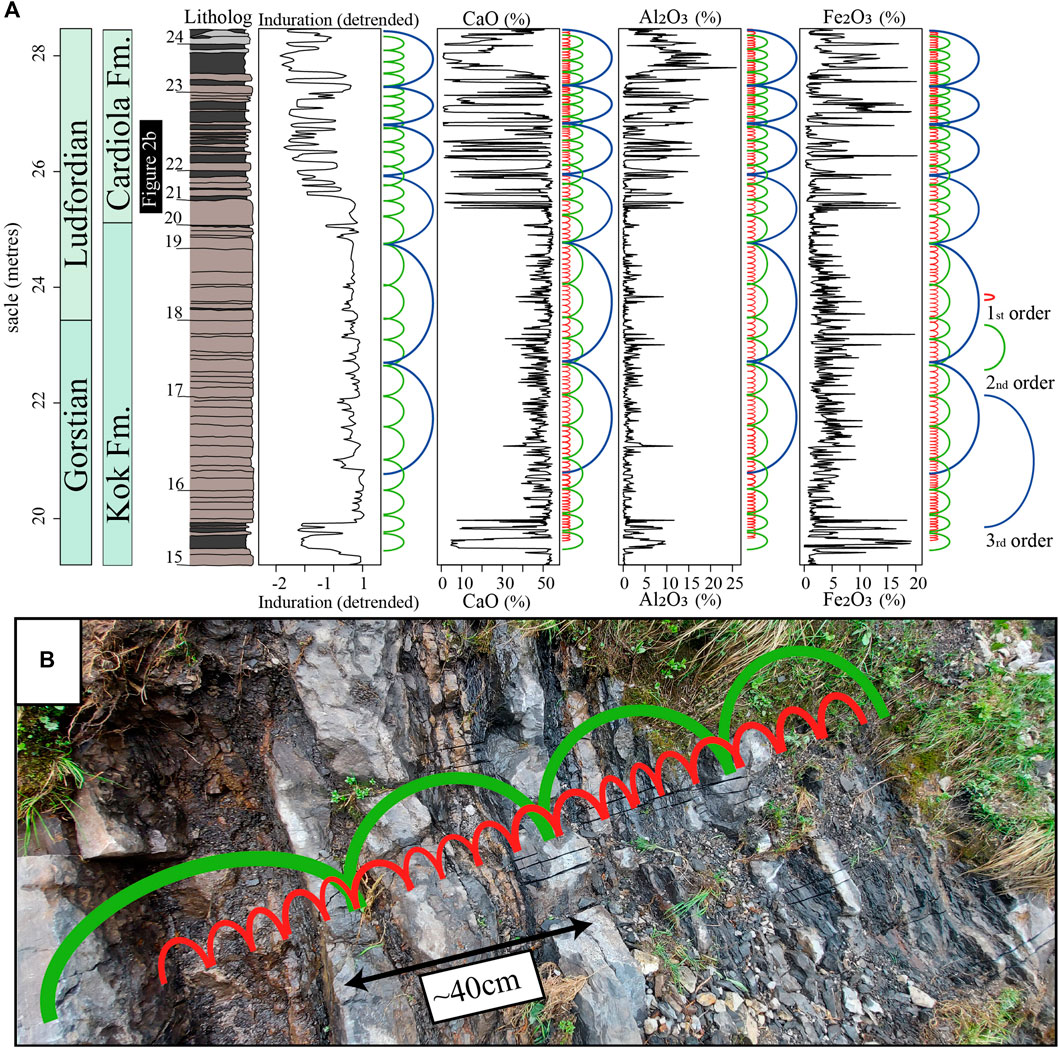
\includegraphics{feart-12-1357751-g005.jpg} \fullcite{arts24aa}
\column{6cm}

\begin{itemize}
\tightlist
\item
  The whole idea of cyclostratigraphy is to identify bundle structures,
  which are organised according to a hiearchy of periods.
\item
  Where does this come from ?
\end{itemize}

\ecolumns
\end{frame}

\hypertarget{the-two-body-problem}{%
\section{The two-body problem}\label{the-two-body-problem}}

\begin{frame}{Suppose the Sun and the Earth are alone in the Univere}
\protect\hypertarget{suppose-the-sun-and-the-earth-are-alone-in-the-univere}{}
\begin{itemize}
\tightlist
\item
  You want to descibe their motion
\item
  The Sun is so big that it is practically the center of mass
\item
  So we take it as the center of our framework. We define a
  \emph{reference plane} and a \emph{reference direction}.
\end{itemize}
\end{frame}

\begin{frame}{The angles and variables describing the orbit (Keplerian
elements)}
\protect\hypertarget{the-angles-and-variables-describing-the-orbit-keplerian-elements}{}
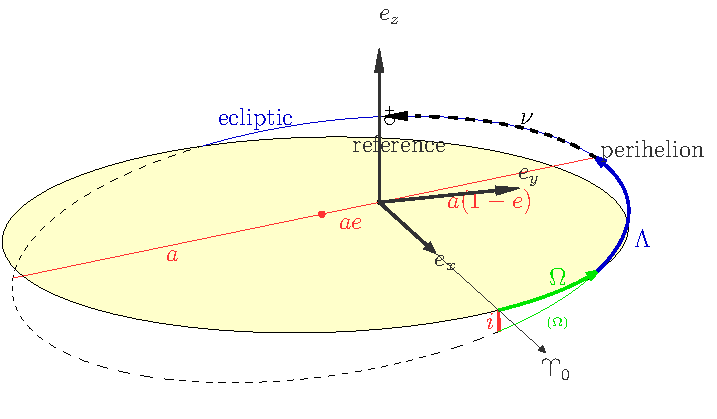
\includegraphics{osculating}
\end{frame}

\begin{frame}{The beauty of the Keplerian orbit}
\protect\hypertarget{the-beauty-of-the-keplerian-orbit}{}
is that all Keplerian elements are constant, except the ``mean
longitude'' \(\ell\), which varies in a somehow tricky way

\begin{itemize}
\item
  Celestial mechanics is an \emph{art} of chosing the right variables to
  make the solution look as simple as possible. Astronomers look for
  \emph{constant of motions} : things that are unchanged along the
  trajectory.
\item
  The approach used since the XIXth century (angle-action) is a bit more
  abstract but the idea is there.
\end{itemize}

\begin{block}{the ``mean longitude'' is linked to angles you can really
measure:}
\protect\hypertarget{the-mean-longitude-is-linked-to-angles-you-can-really-measure}{}
\begin{align*}
\ell &= E - e \sin E.  \\
\tan \frac{\nu}{2} &= \sqrt{\frac{1+e}{1-e}} \tan \frac{E}{2}  
\end{align*}
\end{block}
\end{frame}

\hypertarget{the-linear-perturubation-theory}{%
\section{The linear perturubation
theory}\label{the-linear-perturubation-theory}}

\begin{frame}{You terrified me; why do you say all of this?}
\protect\hypertarget{you-terrified-me-why-do-you-say-all-of-this}{}
\begin{itemize}
\item
  \ldots{} because Sun and Earth are not alone !
\item
  In practice, these equations of \(a\), \(i\) etc. will need to be
  modified to take into account \emph{perturbations} by other planets.
  But how ?
\item
  This ambitious program was developed by Lagrange (1736 -- 1813) and
  Laplace (1749 -- 1827), and many others.
\item
  Astronomers have persued the goal of a \emph{general theory} that
  describes planetary motion is one that is supposed to be valid over a
  \emph{very long} time range : the orbital variables do not go to zero
  or infinity over time.
\end{itemize}
\end{frame}

\begin{frame}{Lagrange and Laplace had already a go!}
\protect\hypertarget{lagrange-and-laplace-had-already-a-go}{}
Indeed ! Already Lagrange and Laplaced introduced the idea of two
abstract vectors (slight re-interpretation):

\begin{itemize}
\tightlist
\item
  the \emph{eccentricity} vector \(\vec{e}\). It has a size \(e\) and
  points to the perihelion.
\item
  the \emph{inclination} vector \(\vec{i}\) : It has a size \(\sin{i}\)
  and points to the ascending node.
\end{itemize}

\textbackslash end\{document\}
\end{frame}

\begin{frame}{The averaging process}
\protect\hypertarget{the-averaging-process}{}
\begin{itemize}
\item
  To make a long (and complicated) story short: we are concerned here
  about mutual interactions of orbital planets over many thousands of
  years. So to first approximation, we care about the mean gravitational
  field generated by a planet over its whole orbit (Gauss' Keplerian
  rings).
\item
  So in a way we are interested about how elements which describe the
  orbit (the ``osculating elements'') influence each other.
\item
  This averaging process is still used today (though not always).
\item
  Laplace and Lagrange found that to a \emph{very first} approximation,
  the movements of \(\vec{e}\) and \(\vec{i}\) can be obtained by
  solving two sets of equations:
\end{itemize}
\end{frame}

\begin{frame}{Linear equations}
\protect\hypertarget{linear-equations}{}
\begin{columns}
\column{6cm}
\[
\begin{pmatrix}
\dot{\vec{e_1}} \\
\dot{\vec{e_2}} \\
\dot{\vec{e_3}} \\
\dot{\vec{e_4}} \\
\dot{\vec{e_5}} \\
\dot{\vec{e_6}}
\end{pmatrix}
= G
\begin{pmatrix}
\vec{e_1} \\
\vec{e_2} \\
\vec{e_3} \\
\vec{e_4} \\
\vec{e_5} \\
\vec{e_6}
\end{pmatrix}
\]
\column{6cm}
\[
\begin{pmatrix}{c}
\dot{\vec{i_1}} \\
\dot{\vec{i_2}} \\
\dot{\vec{i_3}} \\
\dot{\vec{i_4}} \\
\dot{\vec{i_5}} \\
\dot{\vec{i_6}}
\end{pmatrix}
= K
\begin{pmatrix}
\vec{e_1} \\
\vec{e_2} \\
\vec{e_3} \\
\vec{e_4} \\
\vec{e_5} \\
\vec{e_6}
\end{pmatrix}
\]
\end{columns}

where the numbers correspond to the different planets. Nowadays, we call
this an ``eigenvalue'' problem: the vector \(e\) and \(i\) will
oscillate with angular velocities that are the eigenvalues of the
matrices \(G\) and \(K\).
\end{frame}

\begin{frame}{In plain terms:}
\protect\hypertarget{in-plain-terms}{}
This means that given \emph{inital conditions} (which set the phases),
the \(e\) and \(i\) vectors follow quasi periodic movements:

\begin{align*}
e\sin\Pi &= \sum{a_i} \sin{g_i t + \phi_t} \\  
\sin i \sin\Omega &= \sum{b_i} \sin{s_i t + \phi_t} 
\end{align*}

these are the famous \(g\) and \(s\) terms.
\end{frame}

\begin{frame}{Beating}
\protect\hypertarget{beating}{}
\begin{tikzpicture}
  \begin{axis}[
    width=\textwidth,
    height=0.7\textheight,
    axis lines=middle,
    xlabel={$t$},
    ylabel={Amplitude},
    xmin=0, xmax=80,
    ymin=-2.5, ymax=2.5,
    xtick=\empty, ytick=\empty,
    domain=0:80,
    samples=600, 
    xlabel style={at={(axis description cs:1.05,0)}, anchor=west}, % move t further right
    ylabel style={at={(axis description cs:0,1.05)}, anchor=south}, % move Amplitude higher
  ]
    % frequencies
    \pgfmathsetmacro{\fA}{0.25}
    \pgfmathsetmacro{\fB}{0.265}
    \pgfmathsetmacro{\wA}{2*pi*\fA}
    \pgfmathsetmacro{\wB}{2*pi*\fB}
    \pgfmathsetmacro{\wmean}{0.5*(\wA+\wB)}
    \pgfmathsetmacro{\wdiff}{0.5*(\wB-\wA)}

    % individual waves
    \addplot[blue,thin] {sin(deg(\wA*x))};
    \addplot[red,thin] {sin(deg(\wB*x))};

    % sum (beating)
    \addplot[black,thick] {sin(deg(\wA*x)) + sin(deg(\wB*x))};

    % envelopes
    \addplot[dashed,gray] {2*cos(deg(\wdiff*x))};
    \addplot[dashed,gray] {-2*cos(deg(\wdiff*x))};
  \end{axis}
\end{tikzpicture}


\redframetitle
\end{frame}

\begin{frame}{Exercise 1 : Beatings with more periods}
\protect\hypertarget{exercise-1-beatings-with-more-periods}{}
\includegraphics{Png/beatings.png}

\blueframetitle
\end{frame}

\begin{frame}{The beating hiearchy of eccentricity}
\protect\hypertarget{the-beating-hiearchy-of-eccentricity}{}
\redframetitle
\end{frame}

\begin{frame}{Exercise 2 : Understanding the hierarchy of eccentricity
beatings}
\protect\hypertarget{exercise-2-understanding-the-hierarchy-of-eccentricity-beatings}{}
\includegraphics{Png/finding_eccentricity_frequenties.png}

\blueframetitle
\end{frame}

\hypertarget{the-non-linear-perturbation-problem}{%
\section{The non-linear perturbation
problem}\label{the-non-linear-perturbation-problem}}

\begin{frame}{What's wrong with the linear problem}
\protect\hypertarget{whats-wrong-with-the-linear-problem}{}
\begin{itemize}
\item
  Linear theory: perturbations by others orbits, which are considered to
  be non-perturbed
\item
  In reality, they danse together: It implies

  \begin{itemize}
  \tightlist
  \item
    that there are many more possible frequencies than the 8 `g' and `s'
    + background
  \item
    that `g' and `s' move
  \item
    resonances are possible (dancing together). In general: combinations
    of `g' and `s' = 0 are dangerous
  \item
    entering in resonance and resonance escapes are partly inpredictable
  \end{itemize}
\end{itemize}
\end{frame}

\begin{frame}{Mathematical approach (work in progress)}
\protect\hypertarget{mathematical-approach-work-in-progress}{}
\begin{enumerate}
\tightlist
\item
  Analytical approaches :
  \badge{solution = $\sum_i a_i \sin(b_i  t + phi_i )$}

  \begin{itemize}
  \tightlist
  \item
    Historically : Le Verrier, Hill, Bretagnon, and Laskar's thesis Ch.
    1
  \item
    shows of \(g\) and \(s\) combine and contaminate both \(e\) and
    \(i\)
  \item
    Used in the BER78 solution
  \item
    Analytical averaging : Laskar 1988
  \item
    Numerical averaging (Mogaverno and Laskar, using in Hoang et al).
  \item
    First allowed to show resonance, drifts, and cahos
  \item
    by design: respect energy conservation
  \item
    Quinn, Laskar 93 and Laskar 04 (hybrid)
  \item
    Zeebe 2023 (first to be fully open source, based on models
    available)
  \item
    Best to reassess resonances involving the inner planets
  \end{itemize}
\end{enumerate}
\end{frame}

\begin{frame}{Effect of non-linearity: broadening and background}
\protect\hypertarget{effect-of-non-linearity-broadening-and-background}{}
IF I HAVE TIME : SHOW ANALYTICAL VS LA10

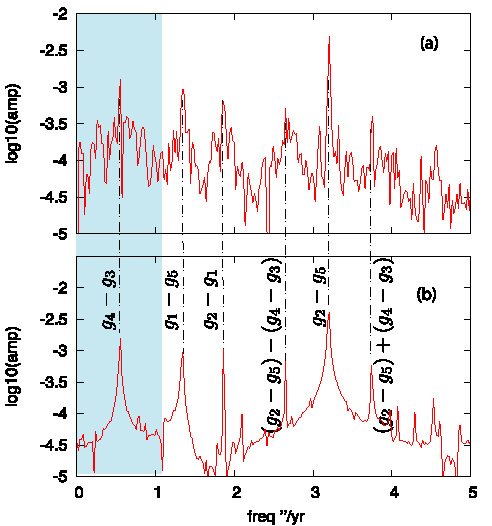
\includegraphics{La10_spectrum_widening.pdf}

\scriptsize\{\fullcite{Laskar11aa} see also exercise by ACDS\}
\end{frame}

\begin{frame}{The (g3-g4) - 2(s3-s4) resonance}
\protect\hypertarget{the-g3-g4---2s3-s4-resonance}{}
\fullcite{Laskar11aa}

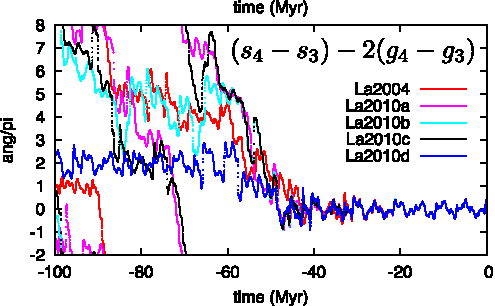
\includegraphics{Figures/La10_resonance_1.pdf}

We introduce here a crucial resonance, which we will further inspect
once we have explained what is obliquity and how it is computed.

\scriptsize\{\fullcite{Laskar11aa} see also qmd exercise 3\}
\end{frame}

\begin{frame}{The 404-ka bomb}
\protect\hypertarget{the-404-ka-bomb}{}
STILL TO DO

\scriptsize\{\fullcite{zeebe24aa}\}
\end{frame}

\hypertarget{the-precession-mouvement}{%
\section{The precession mouvement}\label{the-precession-mouvement}}

\begin{frame}{Climatic precession}
\protect\hypertarget{climatic-precession}{}
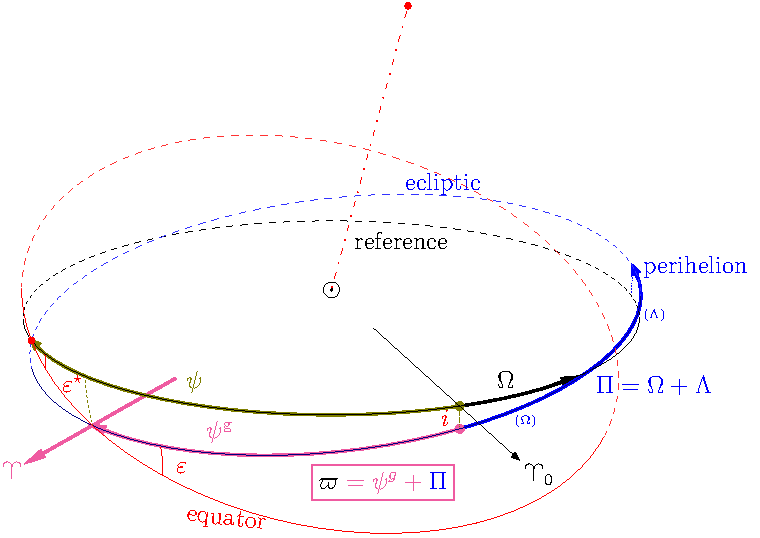
\includegraphics{obliquity}
\end{frame}

\begin{frame}{Climatically relevant}
\protect\hypertarget{climatically-relevant}{}
\begin{itemize}
\tightlist
\item
  What counts, for climate, is insolation that you receive at the
  different \emph{seasons}.
\item
  Seasons depict the course of the \emph{altitude} of the Sun.
\item
  The reference is the point (node) at which the equator and the
  ecliptic intersect (\(\aries\)).
\item
  The relevant angle for precession is thus the \emph{longitude of the
  perihelion} \(\varpi\)
\item
  The relevant angle for ``inclinaison'' is the obliquity
  \(\varepsilon\).
\end{itemize}

\begin{block}{For climate (and cyclostratrigraphy) we care about the
following quantities}
\protect\hypertarget{for-climate-and-cyclostratrigraphy-we-care-about-the-following-quantities}{}
\(\varpi\) : heliocentric longitude of the Sun \(e\) : Eccentricity
\(\varepsilon\) : Obliquity
\end{block}
\end{frame}

\begin{frame}{How does that link to planetary precession ?}
\protect\hypertarget{how-does-that-link-to-planetary-precession}{}
\begin{itemize}
\tightlist
\item
  And to very first order, \emph{general precession} has a regular rate
  of \(k\) = 1 revolution every 23 000 years
\end{itemize}

\begin{block}{What it implies for our frequencies ?}
\protect\hypertarget{what-it-implies-for-our-frequencies}{}
Again, \emph{to very first order} (linear theory)

\begin{itemize}
\tightlist
\item
  Eccentricity: \emph{differences of \(g\) terms}
\item
  \(\varpi\) : \(g + k\) terms
\item
  Obliquity : \(s + k\) terms
\end{itemize}
\end{block}
\end{frame}

\begin{frame}{Obliquity beats}
\protect\hypertarget{obliquity-beats}{}
Obliquity : \(s + k\) terms

Obliquity beats = differences in oblquity terms \(\rightarrow\)
differences in \(s\) terms

Eccentricity beats = differences in precession terms \(\rightarrow\)
differences in \(g\) terms

\redframetitle
\end{frame}

\begin{frame}{Exercise 3 : Visualise the g3-g4 - 2(s3-s4) resonance}
\protect\hypertarget{exercise-3-visualise-the-g3-g4---2s3-s4-resonance}{}
\includegraphics{Png/ob_vs_ecc_beatings.png}
\end{frame}

\begin{frame}{Exercise 3}
\protect\hypertarget{exercise-3}{}
\end{frame}

\begin{frame}{non-linear effects on precession}
\protect\hypertarget{non-linear-effects-on-precession}{}
Looking further general precession \(\psi\) is caused by - the torque by
the Sun and Moon - thus depends (slightly) in \(e\) (for the Earth-Sun
distance) and on the angle between equator and moon orbit - both vary
(the Moon has a constant tilt with respect to the ecliptic\ldots)

\begin{itemize}
\item
  What this says:

  \begin{itemize}
  \tightlist
  \item
    climatic precssion more \emph{variable} when \(e\) is small
    (cf.~Huybers 2008)
  \end{itemize}
\end{itemize}
\end{frame}

\begin{frame}{Mathematical approaches}
\protect\hypertarget{mathematical-approaches}{}
\begin{enumerate}
\tightlist
\item
  Analytical approach (manipulate all terms; use trigonometric laws
  etc.)

  \begin{itemize}
  \tightlist
  \item
    find the origin of all frequencies
  \item
    Sharaf - Budnikova ; Berger's thesis ; R code available from my team
  \end{itemize}
\item
  Numerical integration driven by planetary solution

  \begin{itemize}
  \tightlist
  \item
    e.g.~Laskar and Robutel ; Neron de Surgy (accounts for tidal
    dissipation)
  \item
    Fortran code ; Julia code available from my team.
  \item
    similar approach (based on Quinn) implemented in Zeebe's theme
  \end{itemize}
\end{enumerate}
\end{frame}

\begin{frame}{Resonances and chaos due to precession (also!)}
\protect\hypertarget{resonances-and-chaos-due-to-precession-also}{}
(still to do)
\end{frame}

\begin{frame}{And multi-million-year trend !}
\protect\hypertarget{and-multi-million-year-trend}{}
By its action on tides, the Moon acts as if it was trying to `brake'
(slow-down) Earth's rotation

\begin{itemize}
\tightlist
\item
  Over the years: Earth's slows down and becomes rounder (less torque
  \(\rightarrow\) less precession)
\item
  Moon gains speed \(\rightarrow\) accelerates \(\rightarrow\) escapes
  the Earth
\end{itemize}

This `brake' effect is not constant (it is particluarly high at this
moment; this is not tenable backward in time), prompting evolution
models of dissipation. Resonances are possible.
\end{frame}

\begin{frame}{Two models are currently popular:}
\protect\hypertarget{two-models-are-currently-popular}{}
\bcolumns
\column{6cm}

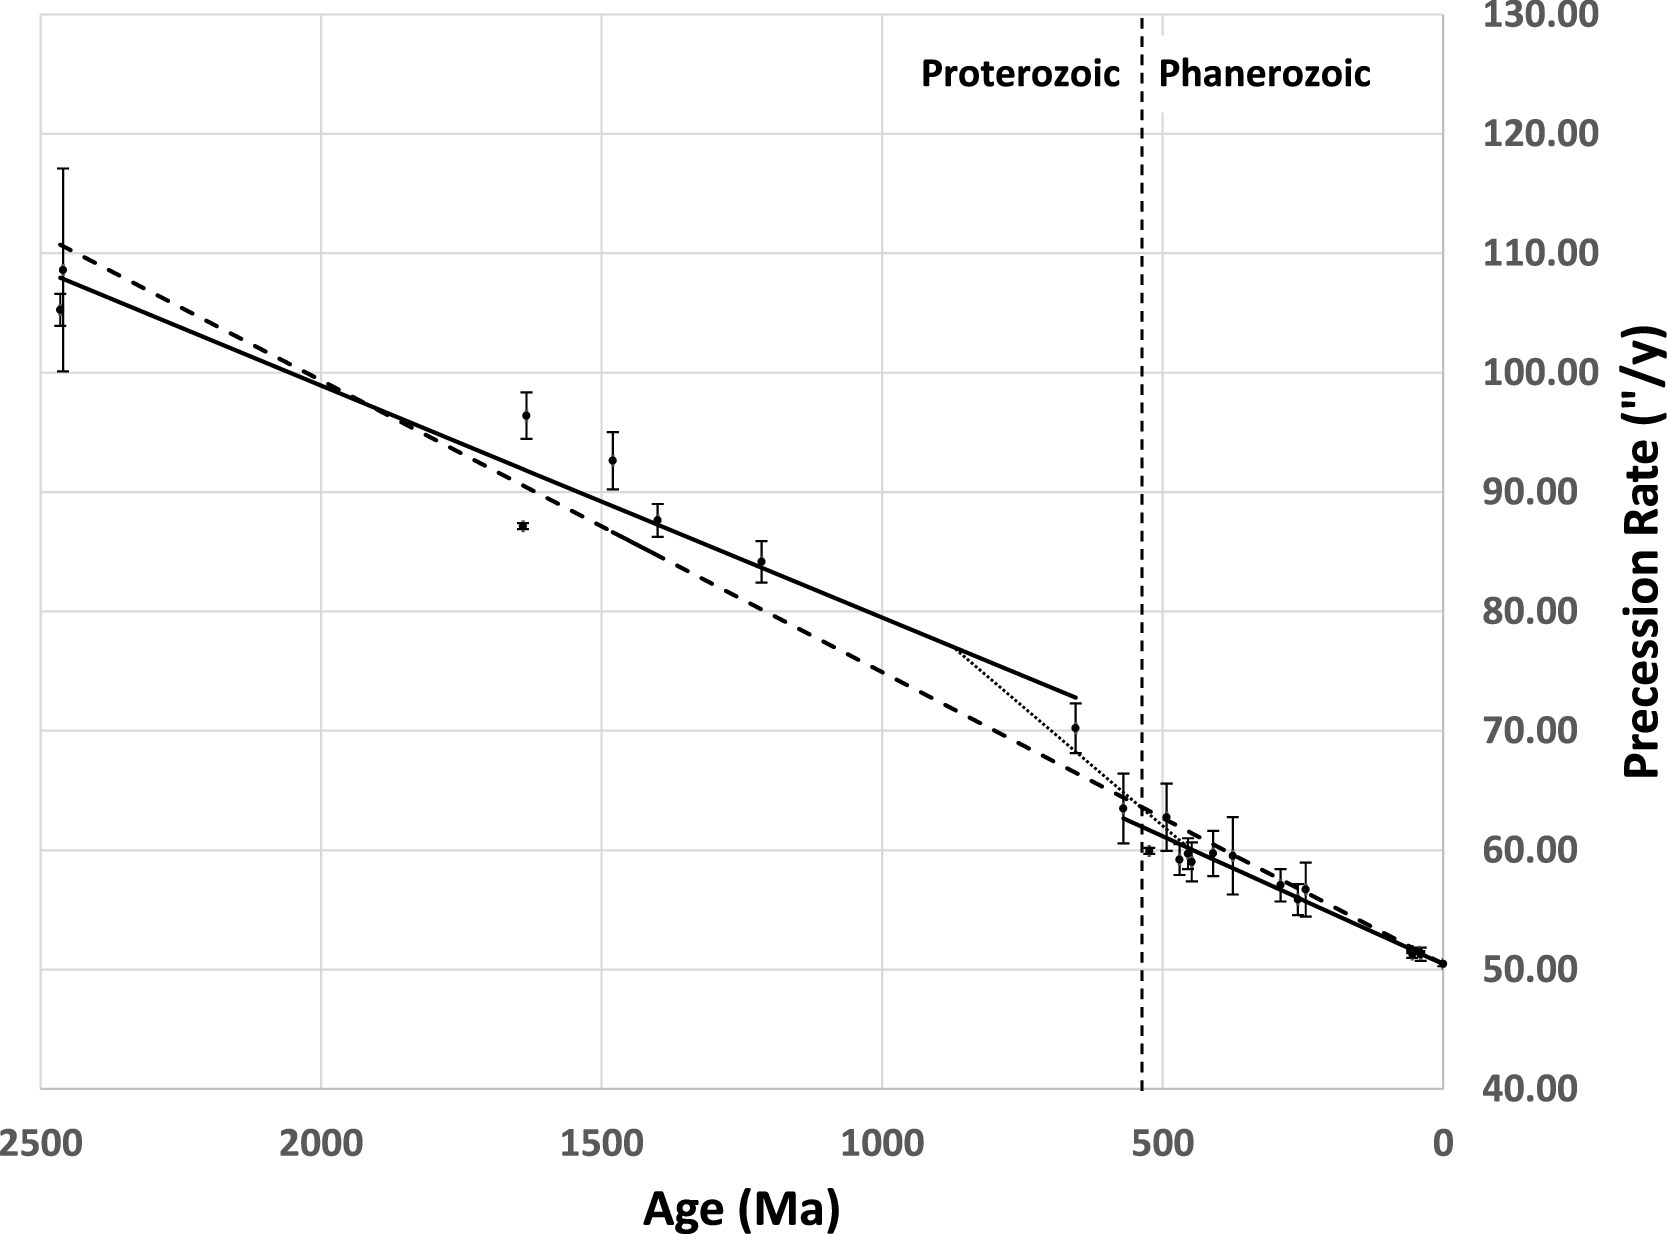
\includegraphics{Figures/Waltham2004.jpg} \fullcite{waltham24aa}

\column{6cm}

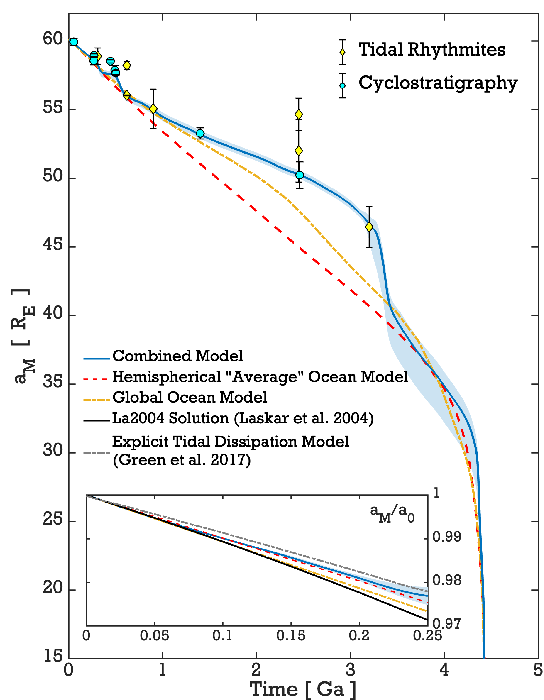
\includegraphics{Figures/2022_Fahrat.pdf} \fullcite{farhat22aa}
\ecolumns
\end{frame}

\begin{frame}{Understand the consequences on the main precession
periods}
\protect\hypertarget{understand-the-consequences-on-the-main-precession-periods}{}
\begin{itemize}
\tightlist
\item
  The periods of eccentricitiy (\(g-\) differences) are unaffected by
  precession (this is planetary)
\item
  The periods of precession (\(g-k\) terms) are (\(k\) is the precession
  rate)
\end{itemize}

Thus the \emph{ratio} gives you an indication on the precession rate. If
you know the LOD, you get the Earth-moon distance.
\end{frame}

 \end{document}


